\documentclass[oneside]{book}

% Load the VUB package.
% This has many options, please read the documentation at
% https://gitlab.com/rubdos/texlive-vub
\usepackage{vub}

% Some highly suggested packages, please read their manuals.
\usepackage{cleveref}
\usepackage[natbib,style=apa]{biblatex}
\addbibresource{../bibliography.bib}
\usepackage{listings}

%space between paragraph and indent all
\setlength{\parskip}{1em}
\usepackage{indentfirst}

%space between bib entries
\setlength\bibitemsep{2\itemsep}

%images settings
\graphicspath{ {./images/} }
\usepackage{graphicx,caption}
\usepackage{float}
\usepackage{rotating}
\usepackage{tikz}

%href package to make references clickable.
\usepackage{hyperref}
\hypersetup{
    colorlinks,
    citecolor=black,
    filecolor=black,
    linkcolor=black,
    urlcolor=black
}

% subfigures
\usepackage{subcaption}

%fix section numbering for use with parts
\renewcommand*\thepart{\Roman{part}}
\makeatletter
\@addtoreset{section}{part}
\makeatother
\renewcommand*\thesection{\arabic{part}.\arabic{section}}
\renewcommand*\thesubsection{\thesection.\arabic{subsection}}

%START title
\title{Computer generated car design}
\subtitle{Assignment 1 - Computational Creativity}
\author{Lennert Bontinck}
\date{February, 2020-2021}
\promotors{Student number: 568702}
\faculty{Computer Science: AI}
\begin{document}
\frontmatter
\maketitle
%END title

%START abstract
\chapter*{Abstract}

% OK

This paper discusses the development and evaluation of a creative system capable of generating photorealistic novel car designs and modifying them.
This system makes use of a pre-trained StyleGAN2 model \citep{stylegan2} and a modified version of the GANSpace tool \citep{ganspace}.
The various components are discussed loosely based on the computational creativity (CC) system description paper by \citet{ventura}.
These components are also placed inside the creative systems framework (CSF) proposed by \citet{csf} to further clarify the creative aspects of the system.

This paper also aims to discuss the possibilities and shortcomings of generative adversarial networks (GANs) in the CC field.
A more philosophical discussion is held to show such systems can indeed be creative rather than just generative.
It is shown how conceptual space exploration tools such as the modified GANSpace tool can be used to combat the black-box problems with GANs.
The need for CC specific internal evaluation and possible solutions are also briefly touched upon.
The external evaluation performed aims to further defend the creativity of the made system and thus the viability of GANs as a creative system.
The used tool for external evaluation was custom build for this project and is made available free to use and open source.

This paper was made as a requirement of the Computational Creativity course taught at the VUB.
All source files for this project are available on GitHub \citep{github_project}.
It is noted that this report is written using a modified version of the VUB based \LaTeX{} template from \citet{latex_template}. 
%END abstract


%TOC
\tableofcontents
\mainmatter

%START MAIN
\part{More technical details}
\label{part:technical_details}


%------------------------------------
\section{Data to be used}
\label{sec:data}

In an ideal scenario, the GAN would make use of custom training data collected for this assignment.
Some technical detail about the required training data, which are images, is given below:
\begin{itemize}
    \item Should be of JPG format.
    \item Should have a maximum resolution of 512x512, preferably even lower (limited computational power).
    \item Should be of cars from a European brand, Peugeot and Mercedes in particular.
    \item Should contain the same car in diverse angles.
    \item Would ideally be labelled with brand, model, colour, body type and release year. The more meta-data the merrier.
    \item From the literature study it seems over 50 thousand images per brand should be needed, \textit{as a minimum}.
\end{itemize}

The images could be scraped from the web.
Thus a custom scraper would need to be written to collect images.
The scraper should work by using popular car auction websites since these would allow for collecting meta-data as well.

While collecting training data for the project would be ideal, this would require a considerable amount of time.
Luckily, if it would turn out unfeasible to do this, many existing pre-bundled training sets exist.
The LSUN-Stanford Car Dataset by \citet{cardb} could be used, as discussed in the previous assignment.
This dataset consists of over 2 million images.

The only drawback of using the LSUN-Stanford Car Dataset is that it consists of images from multiple, mostly American, car brands.
My personal knowledge of these is lesser than my knowledge of European car brands.
This could impose some issues for the evaluation portion of this project since it would be harder to assess if the generated image resembles an existing car.
However, this can be minimized by having enough juries with expertise to evaluate the images.
This will be discussed in greater detail in the next assignment. 

In both of these cases, the used training data would have been already publicly available so there are no expected issues for licensing.


%------------------------------------
\clearpage
\section{Required components and flow of the system}
\label{sec:required_components}

As was already discussed in the previous assignments, the following components are required and will be used from top to bottom:

\begin{itemize}
    \item A crawler that collects input training images from the web.
    \begin{itemize}
        \item Can be bypassed by using LSUN-Stanford Car Dataset.
    \end{itemize}
    \item A DCGAN that generates images of cars based on the collected training images.
    \begin{itemize}
        \item The official TensorFlow implementation of StyleGan2 will be used for this \citep{stylegan2}.
        \item The computational requirement for this is rather gigantic. Luckily a pre-trained car GAN exists as already discussed in the previous assignment. Those could be used as-is or they can be further fine-tuned.
    \end{itemize}
    \item A framework that allows for control over the GAN.
    \begin{itemize}
        \item Since the resulting GAN is of the black-box principle, control over the AI is hard, however, not impossible.
        \item Some research was already done in the previous assignment surrounding control over hidden layers. Since then, a paper that talks about the development of a GUI for this purpose has caught my attention, GANSpace \citep{ganspace}.
        \item GANSpace is compatible with StyleGan2 \citep{ganspace} and supplies an easy-to-use interface.
        \item GANSpace has a demo over the pre-trained StyleGan2 car-related GAN, shown in figure \ref{fig:ganspace}.
    \end{itemize}
    \item An online questionnaire.
    \begin{itemize}
        \item Allows getting human feedback on whether or not the resulting cars look like actual cars.
        \item A tool previously created by me can be modified to hold this survey in a randomised fashion \citep{bapproef}.
        \item More details about this tool will be given in the next assignment.
    \end{itemize}
\end{itemize}

\begin{figure*}
\centering
\begin{subfigure}{.45\textwidth}
  \centering
  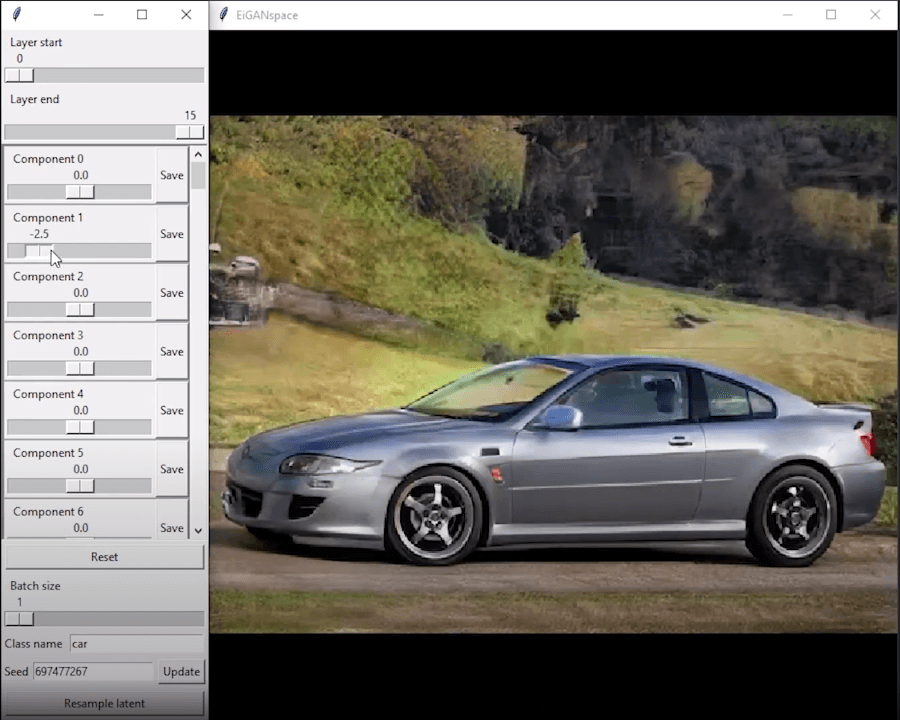
\includegraphics[width=\textwidth]{images/ganspace_1.png}
  \caption{Two door coupe}
  \label{fig:twodoor}
\end{subfigure}%
\hspace{1cm}
\begin{subfigure}{.45\textwidth}
  \centering
  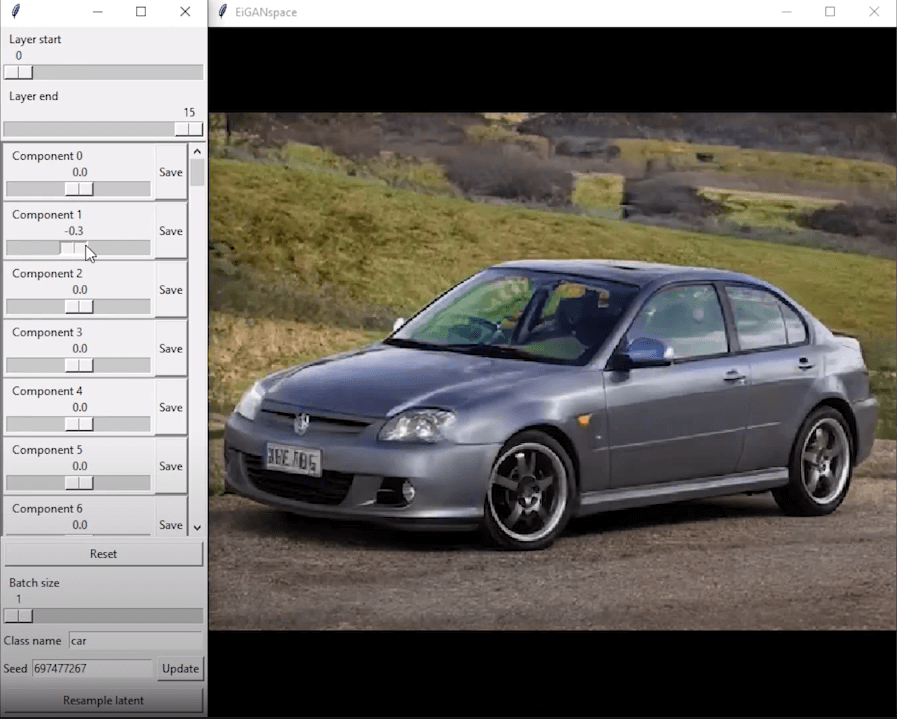
\includegraphics[width=\textwidth]{images/ganspace_2.png}
  \caption{Four door sedan}
  \label{fig:fourdoor}
\end{subfigure}
\captionsetup{width=.85\linewidth}
\caption{Fragments of the GANSpace demo demonstrating the control over the AI to generate similar looking cars with different properties \citep{ganspacevid}.}
\label{fig:ganspace}
\end{figure*}
\part{Conclusions}
\label{part:conclusions}
% wat geleerd en wat onduidelijk

%------------------------------------
\section{Issues this assignment}
\label{sec:issues}

As was discussed in the previous assignment the goal was that a basic version of the GAN would already be implemented by now.
The training process over a subset of the LSUN-Stanford Car Dataset was initiated (using the first 200.000 images) but crashed prematurely. 
It wasn't directly clear why my computer crashed and restarting this process and get a working demo on time for this assignment would not have been possible.
Because of this, this report was shorter and less fine-tuned than the previous ones.
However, a clear understanding of what is needed and how it can be achieved is clearly in place.

%------------------------------------
\section{Expected roadmap}
\label{sec:roadmap}

The following forms an expected roadmap for the remainder of this project:
\begin{itemize}
    \item 23/03 - 02/04: Implementation of the evaluation tool and writing of the evaluation assignment.
    \item 02/04 - 11/04: Development of the GAN.
    \item 11/04 - 15/04: Control over the GAN and collection of images/videos for evaluation.
    \item 15/04 - 29/04: Collection of evaluation data.
    \item 29/04 - 18/05: Writing of the research paper.
\end{itemize}

%references list
\nocite{*}
\printbibliography[heading=bibintoc, title={References}]
\end{document}
